% !TEX program = XeLaTeX
% !TEX encoding = UTF-8 Unicode

%%%%%%%%%%%%%%%%%%%%%%%%%%%%%%%%%%%%%%%%%%%%%%%%
% Multi-Label classification on Apache Spark
%
% License:
% CC BY-NC-SA 3.0 (http://creativecommons.org/licenses/by-nc-sa/3.0/)
%
%%%%%%%%%%%%%%%%%%%%%%%%%%%%%%%%%%%%%%%%%%%%%%%%

%%%%%%%%%%%%%%%%%%%%%%%%%%%%%%%%%%%%%%%%%
% Beamer Presentation
% LaTeX Template
% Version 1.0 (10/11/12)
%
% This template has been downloaded from:
% http://www.LaTeXTemplates.com
%
% License:
% CC BY-NC-SA 3.0 (http://creativecommons.org/licenses/by-nc-sa/3.0/)
%
%%%%%%%%%%%%%%%%%%%%%%%%%%%%%%%%%%%%%%%%%

%----------------------------------------------------------------------------------------
%	PACKAGES AND THEMES
%----------------------------------------------------------------------------------------

\documentclass{beamer}

\mode<presentation> {

% The Beamer class comes with a number of default slide themes
% which change the colors and layouts of slides. Below this is a list
% of all the themes, uncomment each in turn to see what they look like.

%\usetheme{default}
%\usetheme{AnnArbor}
%\usetheme{Antibes}
%\usetheme{Bergen}
%\usetheme{Berkeley}
%\usetheme{Berlin}
%\usetheme{Boadilla}
%\usetheme{CambridgeUS}
%\usetheme{Copenhagen}
%\usetheme{Darmstadt}
%\usetheme{Dresden}
\usetheme{Frankfurt}
%\usetheme{Goettingen}
%\usetheme{Hannover}
%\usetheme{Ilmenau}
%\usetheme{JuanLesPins}
%\usetheme{Luebeck}
%\usetheme{Madrid}
%\usetheme{Malmoe}
%\usetheme{Marburg}
%\usetheme{Montpellier}
%\usetheme{PaloAlto}
%\usetheme{Pittsburgh}
%\usetheme{Rochester}
%\usetheme{Singapore}
%\usetheme{Szeged}
%\usetheme{Warsaw}

% As well as themes, the Beamer class has a number of color themes
% for any slide theme. Uncomment each of these in turn to see how it
% changes the colors of your current slide theme.

%\usecolortheme{albatross}
%\usecolortheme{beaver}
%\usecolortheme{beetle}
%\usecolortheme{crane}
%\usecolortheme{dolphin}
%\usecolortheme{dove}
%\usecolortheme{fly}
%\usecolortheme{lily}
%\usecolortheme{orchid}
%\usecolortheme{rose}
%\usecolortheme{seagull}
%\usecolortheme{seahorse}
%\usecolortheme{whale}
%\usecolortheme{wolverine}

%\setbeamertemplate{footline} % To remove the footer line in all slides uncomment this line
\setbeamertemplate{headline} % To remove the header line in all slides uncomment this line
%\setbeamertemplate{footline}[page number] % To replace the footer line in all slides with a simple slide count uncomment this line

%\setbeamertemplate{navigation symbols}{} % To remove the navigation symbols from the bottom of all slides uncomment this line
}

\usepackage{graphicx} % Allows including images
\usepackage{booktabs} % Allows the use of \toprule, \midrule and \bottomrule in tables
\usepackage{algorithm2e}
\usepackage{fontspec}
\usepackage{xeCJK}

\setCJKmainfont[BoldFont=STHeiti,ItalicFont=STFangsong]{STKaiti}
\hypersetup{colorlinks=false}

%----------------------------------------------------------------------------------------
%	TITLE PAGE
%----------------------------------------------------------------------------------------

\title[MultiBoost]{Multi-Label Classification with Boosting \\ on Apache Spark} 

\author{
白刚  \href{http://weibo.com/baigang111}{@BaiGang-}
} % Your name
\institute[Sina] % Your institution as it will appear on the bottom of every slide, may be shorthand to save space
{
\textit{Sina Ad-Algo}
}
%\date{\today} % Date, can be changed to a custom date
\date{March 21, 2015.} % Date, can be changed to a custom date

\begin{document}

\begin{frame}
\titlepage % Print the title page as the first slide
\end{frame}

\begin{frame}
\frametitle{关于这一文档}
\begin{itemize}
\item TODO: 自我介绍
\item \LaTeX Beamer presentation. 
\item \url{https://github.com/baigang/slides}
\end{itemize}
\end{frame}

\begin{frame}
\frametitle{Overview} % Table of contents slide, comment this block out to remove it
\tableofcontents % Throughout your presentation, if you choose to use \section{} and \subsection{} commands, these will automatically be printed on this slide as an overview of your presentation
\end{frame}

%----------------------------------------------------------------------------------------
%	PRESENTATION SLIDES
%----------------------------------------------------------------------------------------

%------------------------------------------------

\section{背景}

\subsection{The problem}
\begin{frame}
\frametitle{背景:The problem}

  \begin{block}{Business}
   广告为媒体带来收益,同时也潜在的破坏用户体验。
  \end{block}

  \pause

  \begin{columns}[T]
    \begin{column}{.5\textwidth}
      \begin{center}
      
\includegraphics[width=0.8\textwidth]{img/good_ad.png}
      \end{center}
      \begin{center}
      
\includegraphics[width=0.15\textwidth]{img/emoji_smiley.png}
      \end{center}
    \end{column}
    \begin{column}{.5\textwidth}
      \begin{center}
      
\includegraphics[width=0.8\textwidth]{img/bad_ad.png}
      \end{center}
      \begin{center}
      
\includegraphics[width=0.15\textwidth]{img/emoji_unamused.png}
      \end{center}
    \end{column}
  \end{columns}

  \pause

  \begin{block}{}
   不同的广告有不同的受众。\\
   如何将广告投放给其对应的受众?
  \end{block}

\end{frame}

\subsection{User Profiling}

\begin{frame}
\frametitle{背景:User profiling}
\begin{figure}
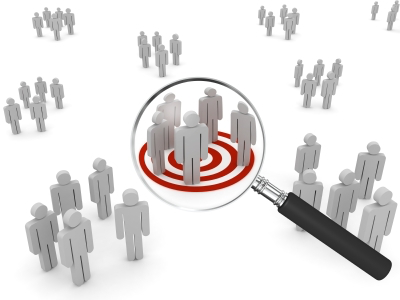
\includegraphics[width=.6\linewidth]{img/target_market.png}
\end{figure}
\begin{block}{理解用户兴趣}
一个用户属于哪个人群,是哪些广告的潜在受众。
\end{block}
\end{frame}

\begin{frame}
\frametitle{背景: User profiling}
\begin{example}{用户兴趣}
  \begin{columns}

   \pause

    \begin{column}{0.333\textwidth}
      \begin{block}{User1}
      \begin{itemize}
        \item 财经-基金
        \item 财经-股票
        \item 房产-装修
        \item ...
      \end{itemize}
      \end{block}
    \end{column}

    \pause

    \begin{column}{0.333\textwidth}
      \begin{block}{User2}
      \begin{itemize}
        \item 休闲-境外游
        \item 娱乐-综艺
        \item 休闲-摄影
        \item ...
      \end{itemize}
      \end{block}
    \end{column}

    \pause

    \begin{column}{0.333\textwidth}
    \begin{block}{User3}
      \begin{itemize}
        \item 体育-足球
        \item 体育-NBA
        \item 游戏动漫
        \item ...
      \end{itemize}
      \end{block}
    \end{column}
  \end{columns}
\end{example}

\pause

用户兴趣是多维度的 $\Rightarrow$ 标签集合 \\
标签是根据business预先设定的 

\pause

\begin{block}{}
我们要解决的实际问题:如何给用户加对应的标签?
\end{block}
\end{frame}

\section{问题与求解}

\begin{frame}
\frametitle{Overview} % Table of contents slide, comment this block out to remove it
\tableofcontents[currentsection] % Throughout your presentation, if you choose to use \section{} and \subsection{} commands, these will automatically be printed on this slide as an overview of your presentation
\end{frame}

\subsection{问题抽象}

\begin{frame}
\frametitle{问题抽象}
\begin{block}{Model and prediction}
根据给出的user feature $\mathbf{x}$,输出符合其兴趣的标签集合$\mathcal{L}$.
$$\mathcal{F} : \mathcal{X} \rightarrow \mathcal{L}$$
\end{block}

\pause

\begin{block}{Model training}
To infer a $\textbf{vector-valued}$ function $\mathcal{F} : \mathcal{X} \rightarrow \mathcal{L}$ from a data set
$$\mathcal{D} = \{({\mathbf{x}}_1, {\mathbf{l}}_1), \cdots, ({\mathbf{x}}_n, {\mathbf{l}}_n)\} \in (\mathcal{X} \times \mathcal{L})^n$$
, where $\mathbf{x} \in \mathcal{R}^d$ and $\mathbf{l} \in {\{+1,-1\}}^L$, by minimizing \textbf{Hamming loss}:
$$\mathcal{Z}_{H} = \frac{1}{\|\mathcal{D}\|} \frac{1}{\|\mathcal{L}\|} \sum_{i=1}^{\|\mathcal{D}\|} \sum_{l=1}^{\|\mathcal{L}\|} \mathfrak{I} [ \mathcal{F}(\mathbf{x}_i)_l \neq \mathbf{y}_{i,l} ]$$
\end{block}
\end{frame}

\begin{frame}
\frametitle{Side note: why not clustering?}

\begin{itemize}
\item 为什么不用Clustering
  \begin{itemize}
    \item Cluster结果 $\neq$  pre-defined labels
    \item 但可以作为user feature
  \end{itemize}
\end{itemize}
\end{frame}

\begin{frame}
\frametitle{Multi-Label classification: Naive方案}

为了得到这个vector-valued function $\mathcal{F} : \mathcal{X} \rightarrow \mathcal{L}$, 我们为每个$\mathit{l} \in \mathcal{L}$ 都训练一个\textit{binary} classifier,预测时将判断每一个标签的结果。

* {\small \color{gray} One-versus-all implemented in LibSVM, scikit-learn, etc.}

\pause

优缺点:
\begin{itemize}
\item 使用已有技术 {  \color{green} \checkmark}
  \begin{itemize}
  \item LR, SVM 等二分类模型
  \end{itemize}
\item 易于验证 {  \color{green} \checkmark}
\item Not (\textit{economically}) scalable  {  \color{red} $\times$}
  \begin{itemize}
  \item num of labels: 10s $\rightarrow$ 10000s 
  \item 逐个训练低效、时间长
  \end{itemize}
\end{itemize}
\end{frame}

\begin{frame}
\frametitle{Multi-label classification: Scalable方案}
目标:
  {
    \setbeamertemplate{itemize items}[checkmark]
    \begin{itemize}
      \item 模型本身的输出就是多标签结果;
      \item 训练过程是最小化Hamming loss;
      \item Scalable.
    \end{itemize}
  }
\pause

方案:
  {
    \setbeamertemplate{itemize items}[square]
    \begin{itemize}
      \item {\color{purple} "Improved Boosting Algorithm Using Confidence-Rated Predictions", Schapire \& Singer, 1999.}
      \begin{itemize}
        \item 提出了AdaBoost.MH算法.
      \end{itemize}
      \item {\color{purple} "The return of AdaBoost.MH: multi-class Hamming trees", Kegl, 2014.}
      \begin{itemize}
        \item Factorization of base learners in AdaBoost.MH.
        \item Decision stump \& Hamming tree作为base learner.
      \end{itemize}
      \item {\color{purple} MultiBoost, http://multiboost.org}
      \begin{itemize}
        \item Open-sourced, single-machine implementations in CPP.
      \end{itemize}
    \end{itemize}
  }
\end{frame}


\subsection{Preliminary: Boosting}

\begin{frame}
\frametitle{Preliminary: Boosting}
\begin{itemize}
\item An additive model. $H(\mathbf{x}) = \sum_i^T \alpha_i h_i(\mathbf{x})$
\item 迭代的在一个 (\textit{re-})weighted sample set上去训练,
\item 通过reweighting,每次训练一个新模型去重点fix前一个模型分类错了的样本
\end{itemize}

\begin{figure}
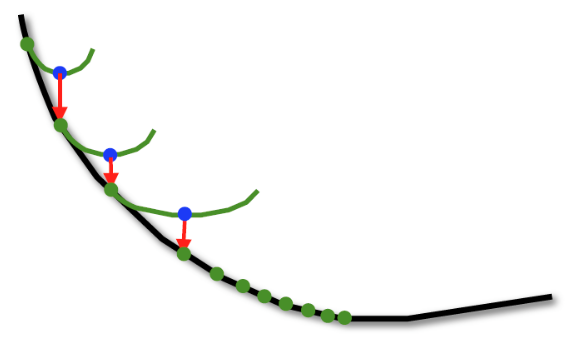
\includegraphics[width=.5\linewidth]{img/boosting.png}
\end{figure}
\end{frame}

\begin{frame}
\frametitle{Preliminary: Adaptive Boosting}

\begin{algorithm}[H]
\SetKwInOut{Input}{input}\SetKwInOut{Output}{output}
 \Input{$\mathcal{D} = (x_i, y_i) \in \{({\mathcal{R}}^n, \{-1, +1\})\}$, $T$, $\mathfrak{B}$}
 \Output{$\mathbf{H} = \Sigma_{t=1}^T{{\alpha}_t {\mathcal{B}}_t}$}
 \Begin{
   ${\mathbf{W}}_1(i) = 1/m$\;
   \For{$t \leftarrow 1, \cdots, T$}{
    ${\mathcal{B}}_t \leftarrow \mathfrak{B}(\mathcal{D}, {\mathbf{W}}_t)$\;
    Get hypothesis set: $h_t \leftarrow \mathcal{B}(\mathcal{D})$\;
    Get the base coefficient ${\alpha}_t$\;
    Update the weights: 
    $${{\mathbf{W}}_{t+1}}(i) = {{{\mathbf{W}}_{t}}(i) \exp(- {\alpha}_t y_i h_t(x_i))} / Z_t $$
    where $Z_t$ is a normalization factor\;
   }
 }
\end{algorithm}

\end{frame}

\subsection{Multi-label boosting}

\begin{frame}
\frametitle{AdaBoost.MH}
\begin{block}{}
\textbf{MH}: \textbf{M}ulti-class with \textbf{H}amming loss.
\end{block}
To produce a \textbf{vector-valued} discriminant function $\mathbf{f}^{(T)} : \mathcal{R}^d \rightarrow \mathcal{R}^K$ with a small Hamming loss $\hat{R}_H (\mathbf{f}^{(T)}, \mathbf{W})$ by minimizing the \textit{weighted multi-class exponential margin-based error}
$$\hat{R}_{EXP}(\mathbf{f}^{(T)}, \mathbf{W}) = \frac{1}{mK} {{\Sigma}_{i=1}^m} {{\Sigma}_{l=1}^K} {\mathbf{W}_{i,l}\exp(- f_l^{(T)} y_{i,l})}$$

The weights $\mathbf{W}$:
$${\Sigma}_{i,l} Wi_{i, l} = 1$$
\end{frame}

\begin{frame}
\frametitle{Exponential loss vs Hamming loss}
\begin{itemize}
\item Exponential loss "upper-bounds" Hamming loss.
  \begin{itemize}
    \item Minimizing exp loss is minimizing Hamming loss.
  \end{itemize}
\item Exponential loss is convex.
  \begin{itemize}
    \item Easy to optimize.
  \end{itemize}
\end{itemize}

\begin{figure}
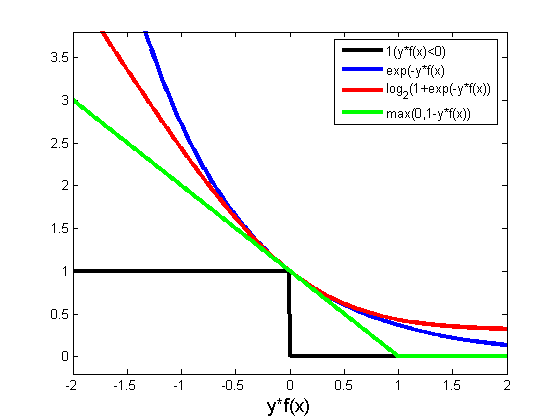
\includegraphics[width=0.6\textwidth]{img/convex-bounds.png}
\end{figure}

\end{frame}

\begin{frame}
\frametitle{AdaBoost.MH}
\begin{algorithm}[H]
\SetKwInOut{Input}{input}\SetKwInOut{Output}{output}
 \Input{$\mathcal{D} = (x_i, y_i) \in $ {\color{blue} $\{({\mathcal{R}}^n, \{-1, +1\}^K\}$ }, $T$, $\mathfrak{B}$}
 \Output{$\mathbf{H} = \Sigma_{t=1}^T{{\alpha}_t {\mathbf{B}}_t} $}
 \Begin{
   {\color{blue} ${\mathbf{W}}_1(i, l) = \frac{1}{mK}$}\;
   \For{$t \leftarrow 1, \cdots, T$}{
    Base learner and the edge: $({\mathcal{B}}_t, \gamma) \leftarrow \mathfrak{B}(\mathcal{D}, \mathbf{W}_t)$\;
    Get hypothesis set: $h_t \leftarrow \mathbf{B}(\mathcal{D})$\;
    Get the base coefficient ${\alpha}_t \leftarrow \frac{1}{2} \exp \frac{1+\gamma}{1-\gamma} $\;
    Update the weights: 
    {\color{blue} $${{\mathbf{W}}_{t+1}}(i,l) = {{{\mathbf{W}}_{t}}(i,l) \exp(- {\alpha}_t y_{i,l} h_t(x_i))} / Z_t $$ }
    where $Z_t$ is a normalization factor\;
   }
 }
\end{algorithm}
\end{frame}

\begin{frame}
\frametitle{AdaBoost.MH}
将minimizing exp-loss:
$$\hat{Z}(\mathbf{f}^{(T)}, \mathbf{W}) = \frac{1}{mK} {{\Sigma}_{i=1}^m} {{\Sigma}_{l=1}^K} {w_{i,l}\exp(- f_l^{(T)} y_{i,l})}$$
转化成maximizing "the edge":
$$ \gamma(\mathbf{W}, y, \mathbf{p}) = \Sigma_{i=1}^{n} \Sigma_{l=1}^{L} \mathbf{W}_{i,l} * y_{i,l} * \mathbf{p}_{i, l}$$
其中,$\mathbf{W}$是权重,$y$是label,$p$是prediction,$p \in \{-1, +1\}$。
\end{frame}

\begin{frame}
\frametitle{The base learner factor}
\begin{block}{The EXP loss:}
$$Z(\mathbf{h}, \mathbf{W}) = \sum_{i=1}^{n} \sum_{l=1}^{K} w_{i,l} \exp(-\mathcal{B}_{i,l} y_{i,l}) $$
$$= \frac{e^\alpha + e^{-\alpha}}{2} - \frac{e^\alpha - e^{-\alpha}}{2} \gamma$$
\end{block}
\begin{block}{$\alpha$ minimizing the EXP loss:}
$$\alpha = \frac{1}{2} \log \frac{1+\gamma}{1-\gamma}$$
\end{block}
\end{frame}

\begin{frame}
\frametitle{Factorization of base learners}
便于计算$\gamma$,把general vector-valued function $\mathcal{B}$ 分解
\begin{itemize}
\item $\varphi(x)$: a \textit{label independent} scalar function
\begin{itemize}
  \item 本质上是对\textit{feature space}做划分
\end{itemize}
\item $\mathbf{v}$: a \textit{feature independent} vector-valued function
\begin{itemize}
  \item 将$\varphi(x)$划分的二元或者多元结果cast到\textit{label space}上
  \item "output encode"
\end{itemize}
\end{itemize}

$$\mathcal{B}(\mathbf{x}) = \varphi(\mathbf{x}) \mathbf{v})$$

\end{frame}

\begin{frame}
\frametitle{Base learner training}
\begin{itemize}
\item 求$\varphi(x)$:按照什么原则对feature space做划分
\item 求$\mathbf{v}$:如何最优的"cast to labels"

\pause

\begin{block}{}
Maximizing "the edge" $\gamma$.
\end{block}

\pause

\end{itemize}
      {\color{purple} "The return of AdaBoost.MH: multi-class Hamming trees", Kegl, 2014.}
{
  \setbeamertemplate{itemize items}[checkmark]
  \begin{itemize}
    \item Tree-based方案:$\varphi(x)$是Decision stump/Hamming tree
    \item $\mathbf{v}$与$\varphi(x)$同时优化求解
  \end{itemize}
}
\end{frame}

\begin{frame}
\frametitle{Base learner: the Decision Stump model}
\begin{itemize}
\item Decision stump: 一个只有一个结点的分类树
$$ \varphi_{j,b}(\mathbf{x}) = \left\{
  \begin{array}{l l}
    1 & \quad \text{if } \mathbf{x}_j \geq b, \\
    -1 & \quad \text{otherwise.}
  \end{array} \right.$$
\item Hamming Tree
\begin{itemize}
  \item Decision stump作为内部结点的树
\end{itemize}
\end{itemize}
\end{frame}


\begin{frame}
\frametitle{Base learning}

"Edge" $\gamma$ 是 per-class edge的和。
$$\gamma = \Sigma_l \gamma_l, \gamma_l = \Sigma_{i=1}^n \mathbf{W}_{i,l} \mathbf{p}_{i,l} y_{i,l} $$
$$ \gamma_l = \Sigma_{i=1}^{n}\mathbf{W}_{i,l}\mathfrak{I}\{\mathbf{p}_{i,l} = y_{i,l}\} - \Sigma_{i=1}^{n}\mathbf{W}_{i,l}\mathfrak{I}\{\mathbf{p}_{i,l} \neq y_{i,l}\} $$

\pause

The \textit{weighted per-class error rate}
$$\mu_{l-} = \sum_{i=1}^{n}w_{i,j}\mathfrak{I}\{\varphi(\mathbf{x}_i) \neq y_{i,l}\}$$
The \textit{weighted per-class correct classification rate}
$$\mu_{l+} = \sum_{i=1}^{n}w_{i,j}\mathfrak{I}\{\varphi(\mathbf{x}_i) = y_{i,l}\}$$

\pause

$$\gamma_l = \mu_{l+} - \mu_{l-}$$

\end{frame}

\begin{frame}
\frametitle{Base learning}

\begin{block}{Find $\varphi(\bullet)$ by maximazing the full edge $\gamma$}
\begin{itemize}
\item Decision Stump: finding the best split cut
\item Hamming tree: node split with the max edge improvement
\item Generalized binary classifier.
\end{itemize}
\end{block}

\begin{block}{Given $\varphi(\bullet)$, set the votes vector $\mathbf{v}$}
$\mathbf{v}$ maximizing the full edge is:
\[v_l = \left\{
  \begin{array}{l l}
  1 \quad \quad \text{   if } \mu_{l+} > \mu_{l-} \\
  -1 \quad \text{ otherwise }
  \end{array} \right. \]
\end{block}

\end{frame}

\section{Multiboost on Spark}

\subsection{Base learner: Decision Stump}

\begin{frame}
\frametitle{Decision stump}
\end{frame}

\begin{frame}
\frametitle{Decision stump on Apache Spark}
\end{frame}

\subsection{Base learner: generalized binary classifier with vote vector}

\begin{frame}
\frametitle{Generalized binary classifier as $\varphi(\dot)$}
\end{frame}

\begin{frame}
\frametitle{Generalized binary $\varphi$ on Apache Spark}
\end{frame}


\subsection{Strong learner: Iterative runner}

\begin{frame}
\frametitle{Strong learner}

\end{frame}

%----------------------------------------------------------------------------------------

\subsection{实验与效果}

\begin{frame}
\frametitle{Experiments setup}
\begin{itemize}
\item 数据集来源 -- 内部、外部通用测试集
\item 集群环境 TODO
\end{itemize}
\end{frame}

\begin{frame}
\frametitle{运行时间}
TODO: 对应数据集的训练时间长度
\end{frame}

\begin{frame}
\frametitle{效果}
\begin{itemize}
\item 对应数据集的训练和测试error,有图
\end{itemize}
\end{frame}


\subsection{后续工作}

\begin{frame}
\frametitle{后续工作}
\begin{itemize}
\item 使用LR、SVM作为$\varphi$,其loss与edge-maximizing目标一致需要理论证明
\item 训练数据中允许有missing data
\item 现有时间基于Spark 1.1.x, 应用新的spark ml interface
  \begin{itemize}
    \item $\star \star \star$ 欢迎'Fork and Star'!
  \end{itemize}
\end{itemize}
\end{frame}

\end{document} 
